The \emph{Dirichlet} boundary condition is enforced before and directly after the projection step. Our implementation loops over the grid containing information on solid cells. If for example a solid is present at grid index \emph{(i,j,k)} defined at the center of the grid cell, all velocities in the staggered MAC grids for the fuel and hot gaseous products sharing a cell wall with \emph{(i,j,k)} are set to zero, projecting the velocity vector onto the tangent plane of the cell surface. This results in that no velocity vectors point into cells that are solid, making sure that no fluid will flow into solid objects.

\begin{figure}[H]
\centering
\subfigure[before]{\centering
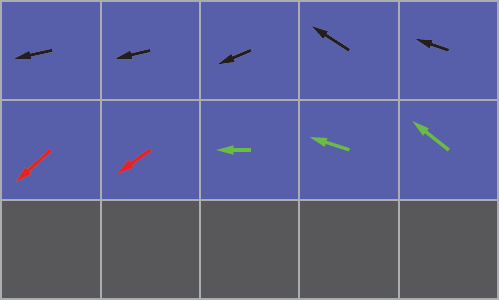
\includegraphics[width=.45 \linewidth]{figures/dirichlet_before.png}
}
\subfigure[after]{\centering
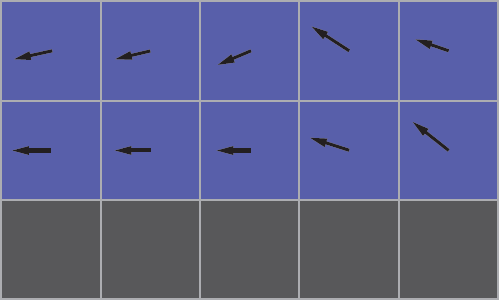
\includegraphics[width=.45\linewidth]{figures/dirichlet_after.png}
}
\caption
{
\label{fig:dirichlet_boundary_condition}
Velocity vectors before and after enforcing the Dirichlet boundary condition. Image courtesy of \emph{TNM079, LiU}.
}
\end{figure}

The \emph{Neumann} boundary condition is enforced when building the Poisson matrix during the projection step. If we for a fluid cell find a neighbouring solid cell, that solid cell's entry in the diagonal matrix is set to zero. This ensures that no exchange of fluid will take place between the fluid cell and the cell marked as solid.

\begin{figure}[h!]
\label{fig:neumann_boundary_condition}
\centering
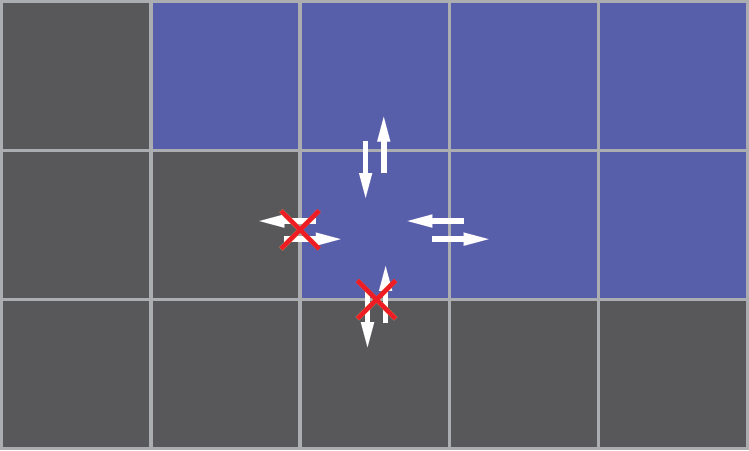
\includegraphics[width=0.4\textwidth]{figures/neumann_condition.png}
\caption{ The Neumann boundary condition ensures no fluid exchange between solid- and fuel cells. Image courtesy of \emph{TNM079, LiU}.}
\end{figure}